\RequirePackage{plautopatch}
\RequirePackage[l2tabu, orthodox]{nag}

\documentclass[uplatex,dvipdfmx]{jlreq}
\usepackage{osukalab2020}
\usepackage{epic,eepic}
\usepackage{graphicx}
\usepackage{amsmath}
\usepackage[all, warning]{onlyamsmath}
\usepackage{siunitx}
\usepackage{txfonts}
\usepackage{amssymb}
\usepackage{comment}


\pagestyle{empty}

\headding{大須賀・杉本研 研究会資料}
\title{脚型壁面歩行ロボットの開発と性能実験}
\author{吉田壱平}
%\abstract{}
%\keywords{}

\begin{document}
\maketitle
\thispagestyle{empty}
\section{緒言}

\begin{comment}
第一案
災害や化学テロの現場調査などの人間が立ち入るのが困難な場所においては,人間の代わりに災害探査ロボットの活躍が期待されている~\cite{大須賀公一2004ヘビ型ロボットによる狭空間探索}.
現在は,災害探査ロボットとしてクローラ型を採用しているものが多い~\cite{高森年2003災害における罹災者発見とクローラ型ロボット,久武経夫2011大災害に立ち向かうロボットの開発}.
クローラ型は広い接地能力による駆動力と,その柔軟性による不整地対応性において瓦礫の積もる場所などでの,災害探査ロボットの移動手段として有用である~\cite{小柳栄次2010サブクローラを持つレスキューロボット}.
その一方で,ビルなど高層建造物や高所の探索においては,建物内の階段などを登ってアプローチするのではなく,壁面や天井を直接移動することで,素早く内部の情報を得ることができるので,災害探査ロボットの一つの形態として壁面歩行ロボットに有用性があると考えられる.

今日に至るまで壁面歩行ロボットというのは様々な形で実現されてきた.
その吸着機構としては,吸盤などの負圧を利用するもの~\cite{広瀬茂男1991四足壁面移動ロボット},磁力を利用するもの~\cite{高田洋吾2013立体的な環境で活動できる橋梁検査ロボットの開発},プロペラなどによるダウンフォースを利用するもの~\cite{weko_4205_1}などがある.
磁力式は強力な吸着力によって磁力を持つ平面上での作業ロボットとして有用である~\cite{高田洋吾2013立体的な環境で活動できる橋梁検査ロボットの開発}.しかし,吸着できる面が磁力を持つものに限られるという課題がある.
また,迅速な対応の求められる災害現場においてはプロペラ式の速度は有用であるが\cite{weko_4205_1},吸着の安定のための制御器への負担と,風などの外部環境の影響を受けることに課題がある~\cite{西亮1991推進力による壁面移動ロボットの研究,鈴木隆宏2009g1501}.
よって本研究においては,吸着面の材質を選ばず,吸着面との機密性を保つことができれば,安定的な吸着力を発揮することのできる負圧式を吸着機構として選択した.

現存する負圧式の壁面歩行ロボットはその移動方法を大きく,吸着式クローラ型~\cite{福田敏男1994壁面走行ロボットの研究}と脚型~\cite{広瀬茂男1991四足壁面移動ロボット}に分けることができる.
一般に,吸着式クローラ型は移動速度において脚型よりも優れているが\cite{福田敏男1992壁面走行ロボッ},脚型は脚の設置面を選択できるので,吸着のしにくい凹凸や亀裂を避けて移動することができる.
以上のことから本研究では負圧による吸着機構を有する脚型の壁面歩行ロボットの製作を目指す.
その壁面歩行ロボット製作に向けて本研究ではまず,壁面のみを移動することのできる脚型壁面歩行ロボットの開発と性能実験に取り組んだ.

\end{comment}

現代社会において,屋内で移動や作業をするロボットが様々な面から必要とされているのは言うまでも無い.
その際の移動方法としては移動用クローラ~\cite{小柳栄次2010サブクローラを持つレスキューロボット}や車輪~\cite{尾崎功一20082p2}を利用したものなどがある.
これらの移動ロボットは地面の凹凸などに柔軟に対応し,高い踏破性を持つが,人間の生活する屋内を移動する上では,階段などの段差が大きな障害となる.
クローラ型のロボットの中にはそういった段差の問題を,2つのクローラ機構を有することによって解決している物もあるが~\cite{小柳栄次2010サブクローラを持つレスキューロボット},越えることのできる段差の大きさがクローラの大きさに依存してしまうという課題を抱えている.
移動機構が大きくなるということは,結果的にそのロボットの活動範囲を縮めてしまうことになる.そこで,移動機構の大きさに依存せず段差を踏破できることのできるロボットを開発することで,活動範囲を縮めずに屋内の移動をするロボットの開発を目指す.
本研究では,そのような移動機構を持つロボットとして壁面歩行ロボットの開発を行う.

階段のような段差も広く捉えれば壁であり,その壁面に吸着し移動することで段差などの踏破を実現する.
また,凹凸や亀裂など壁面の状況によっては吸着による移動が難しいこともある.
そこで,凹凸などへも対応することのできる吸着機構の開発を目指しつつ,段差への吸着がどうしても不可能な場合は屋内の別の壁面を利用してその段差を越えるなど,様々なルートの選択が可能になるロボットの開発ができればより有用である.

今日に至るまで壁面歩行ロボットというのは様々な形で実現されてきた.
その吸着機構としては,吸盤などの負圧を利用するもの~\cite{広瀬茂男1991四足壁面移動ロボット},磁力を利用するもの~\cite{高田洋吾2013立体的な環境で活動できる橋梁検査ロボットの開発},プロペラなどによるダウンフォースを利用するもの~\cite{weko_4205_1}などがある.
磁力式は強力な吸着力によって磁力を持つ平面上での作業ロボットとして有用である~\cite{高田洋吾2013立体的な環境で活動できる橋梁検査ロボットの開発}.しかし,吸着できる面が磁力を持つものに限られるという課題がある.
また,プロペラ式は移動の速さに利点があるが~\cite{weko_4205_1},吸着の安定のための制御器への負担と,風などの外部環境の影響を受けることに課題がある~\cite{西亮1991推進力による壁面移動ロボットの研究,鈴木隆宏2009g1501}.
よって本研究においては,吸着面の材質を選ばず,吸着面との機密性を保つことができれば,安定的な吸着力を発揮することのできる負圧式を吸着機構として選択した.

現存する負圧式の壁面歩行ロボットは,その移動方法を大きく吸着式クローラ型~\cite{福田敏男1994壁面走行ロボットの研究}と脚型~\cite{広瀬茂男1991四足壁面移動ロボット}に分けることができる.
一般に,吸着式クローラ型は移動速度において脚型よりも優れているが\cite{福田敏男1992壁面走行ロボッ},脚型は脚の設置面を選択できるので,吸着のしにくい凹凸や亀裂を避けて移動することができる.
以上のことから本研究では負圧による吸着機構を有する脚型の壁面歩行ロボットの製作を目指す.
その壁面歩行ロボット製作に向けてまずは,壁面のみを移動することのできる脚型壁面歩行ロボットの開発と性能実験に取り組んだ.


\begin{figure}[t]
    \centering
    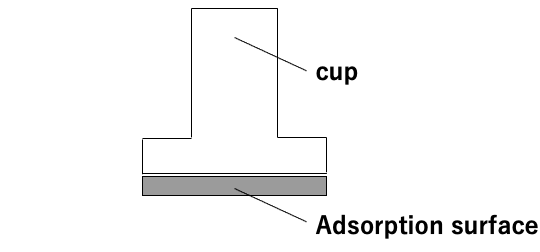
\includegraphics[height=40mm,]{./figure/sideview_sucker.png}
    \caption{Model of the sucker seen from the side.}
    \label{fig:model_sucker}
\end{figure}

\section{負圧を用いた吸着機構の製作}
\subsection{ロボットの構成}
製作した4足歩行ロボットの模式図をFig.~\ref{fig:model_of_the_quadruped}に示す.機体は負圧による吸着力を生み出す吸着部とサーボモータによって4足歩行運動を生み出す胴体部の2つに分けられる.
その内,本章では吸着部について述べる.

\begin{figure}
    \centering
    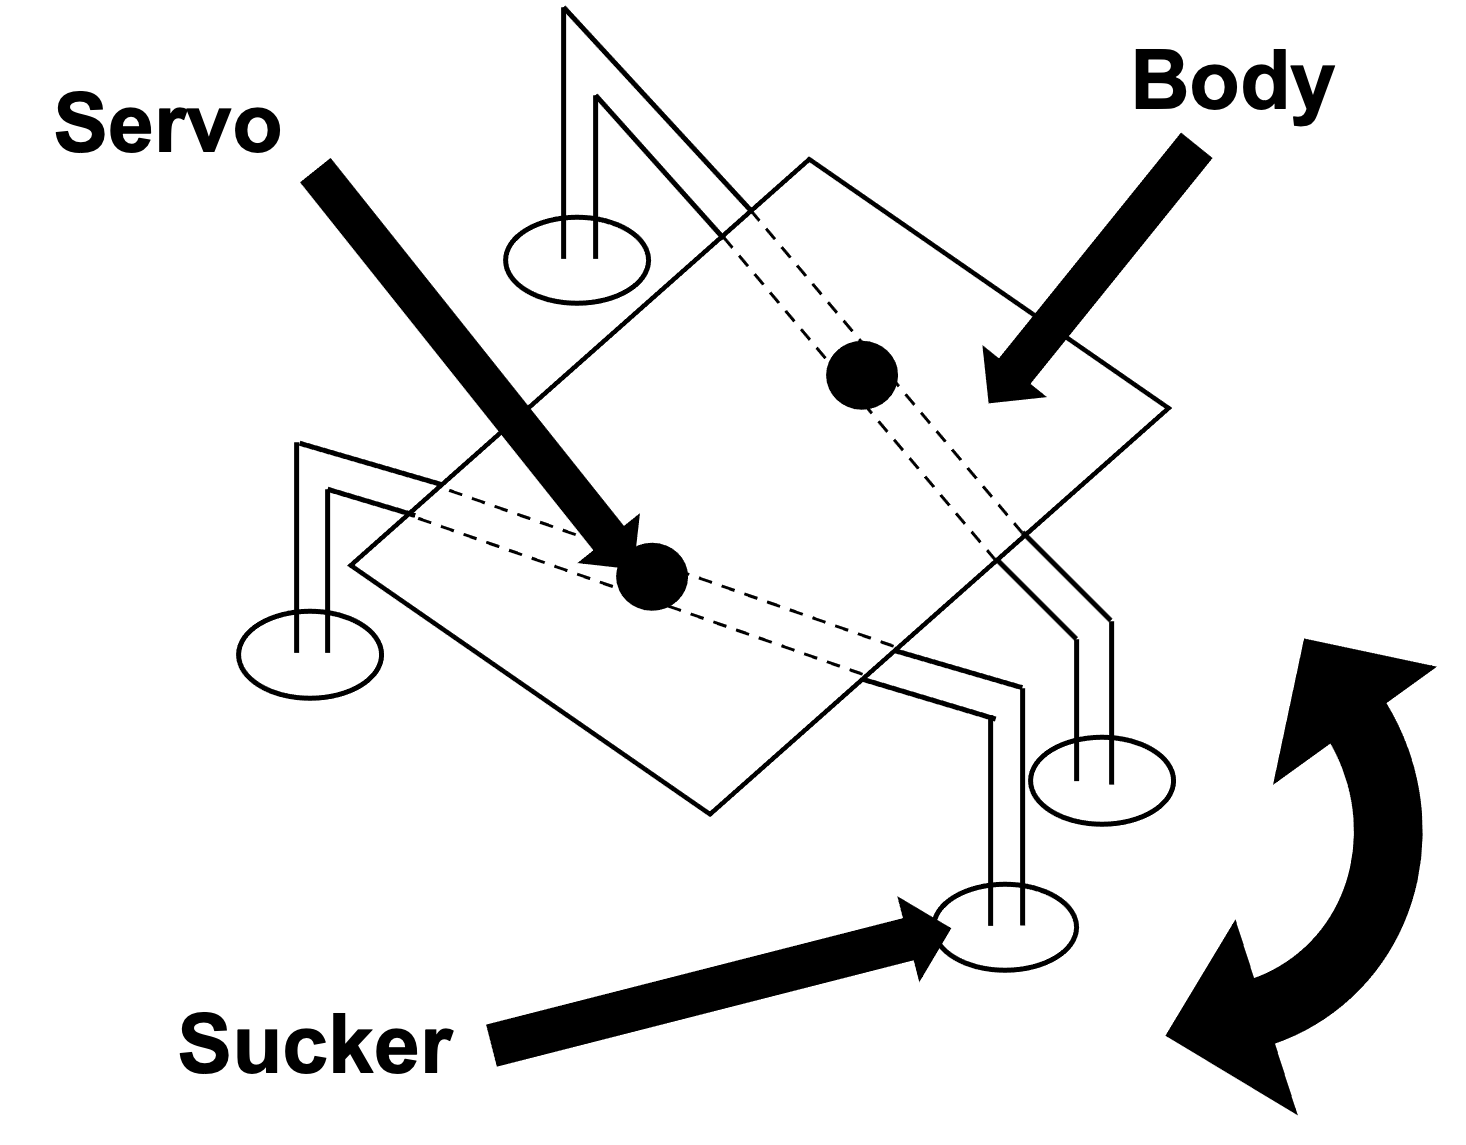
\includegraphics[width=60mm]{./figure/overview_model.png}
    \caption{Model of the quadruped.}
    \label{fig:model_of_the_quadruped}
\end{figure}

\subsection{吸盤の製作}
負圧を発生させるための吸盤については,後述するゲル性の接面部への接着のしやすさやと,脚部分との接続のしやすさ,またその面積や形状を自由に変えられるという点を考慮して,自作することにした.
また,便宜上Fig.~\ref{fig:model_sucker}に示すように吸盤の本体を椀状部(cup),壁面に接する部分を接面部(Adsorption surface)とする.
\subsubsection{椀状部の製作}
椀状部の製作にはウェーブ・シリコーンゴム(ウェーブ社製)を用いた.接面部との接着を考え椀状部のFig.~\ref{fig:model_sucker}における下面は平面にし,脚部との接続のため,椀状部の上側に突起をつけた.
製作した椀状部をFig.~\ref{fig:siliconsucker}に示す.

\begin{figure}[tb]
    \begin{tabular}{cc}
    \begin{minipage}{0.45\hsize}
      \centering 
      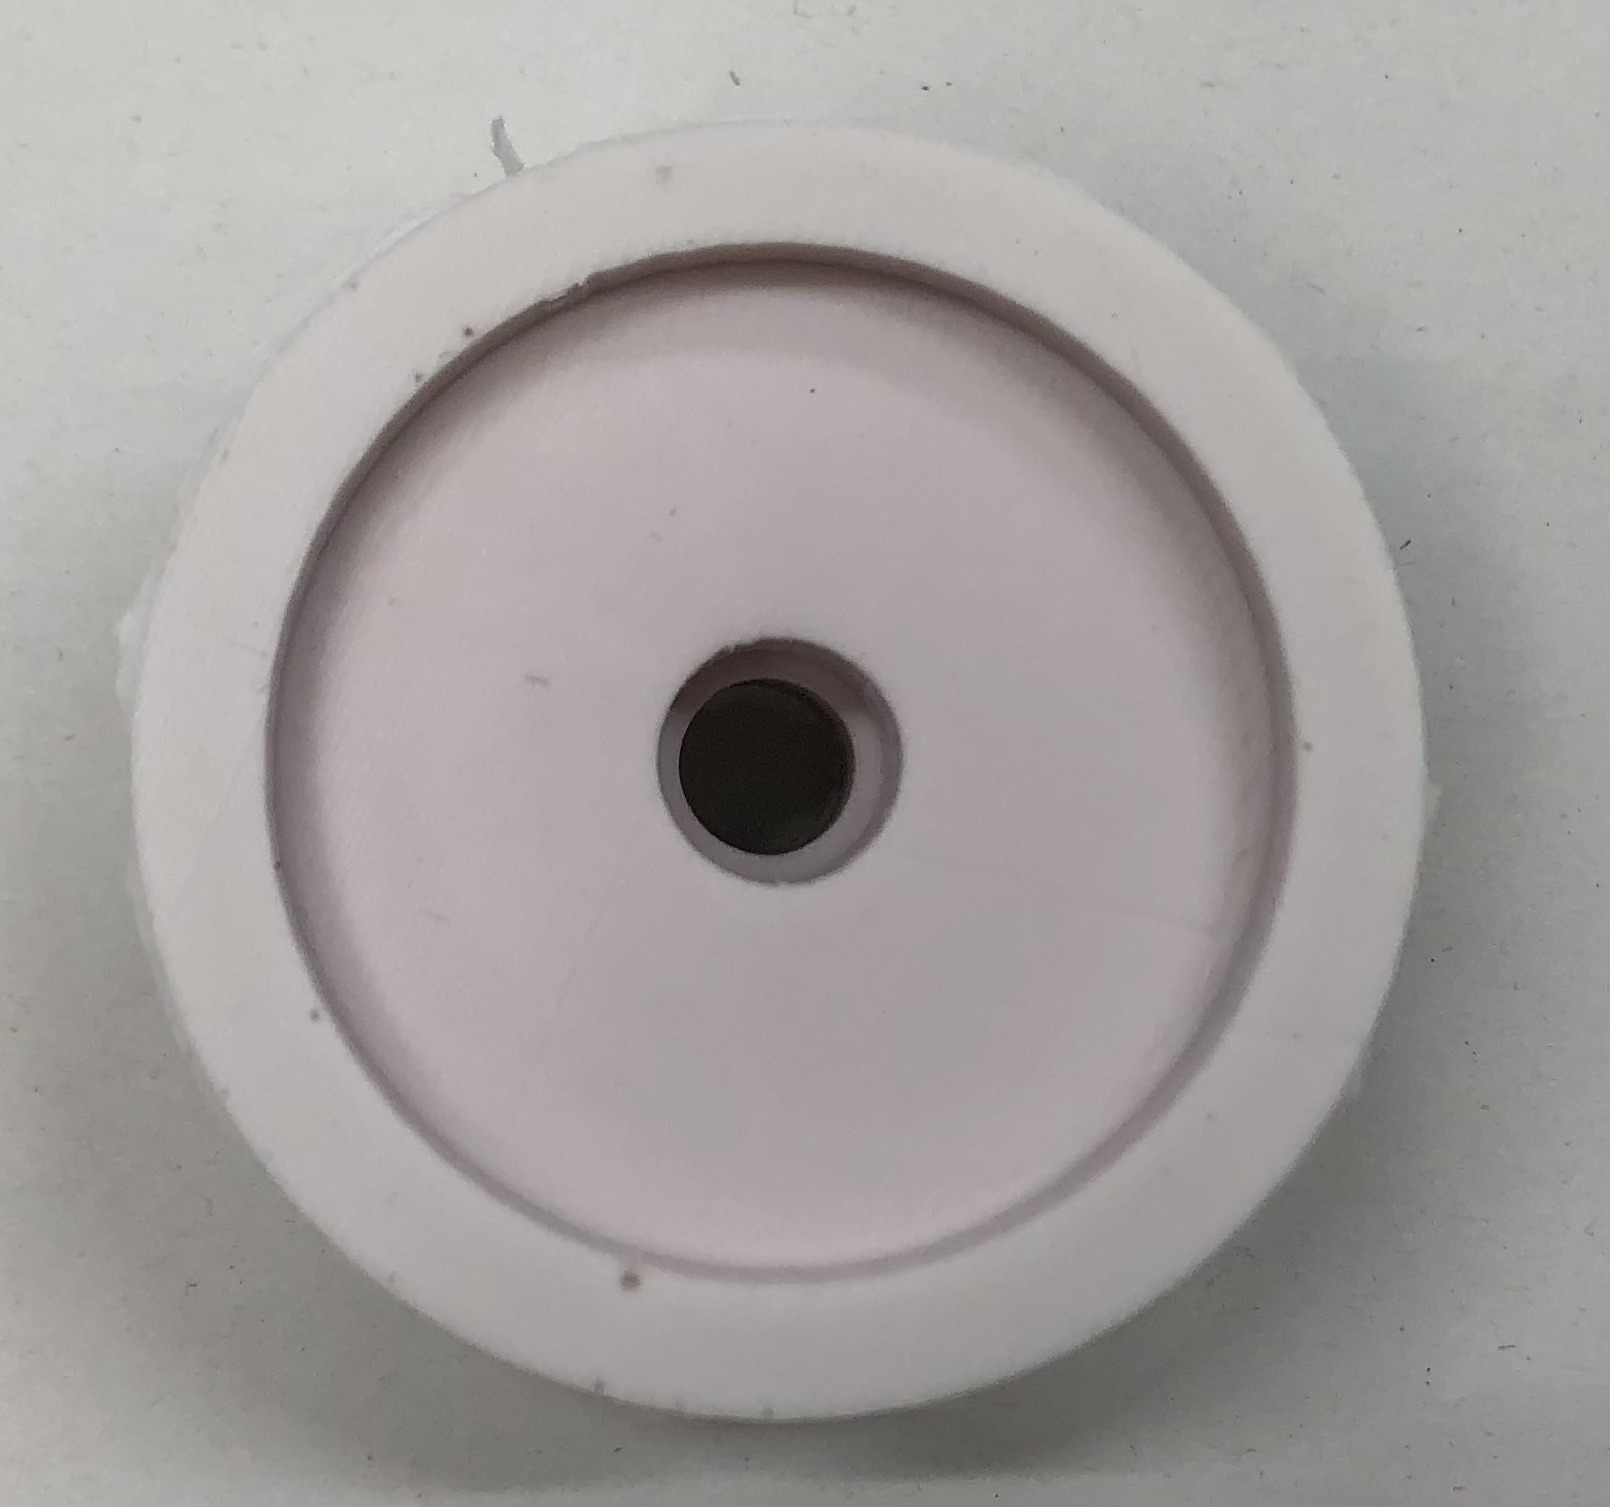
\includegraphics[width=\columnwidth]{./figure/sucker_botm.jpg}
      \subcaption{Adsorption surface.}
    \end{minipage}
    \begin{minipage}{0.45\hsize}
      \centering 
      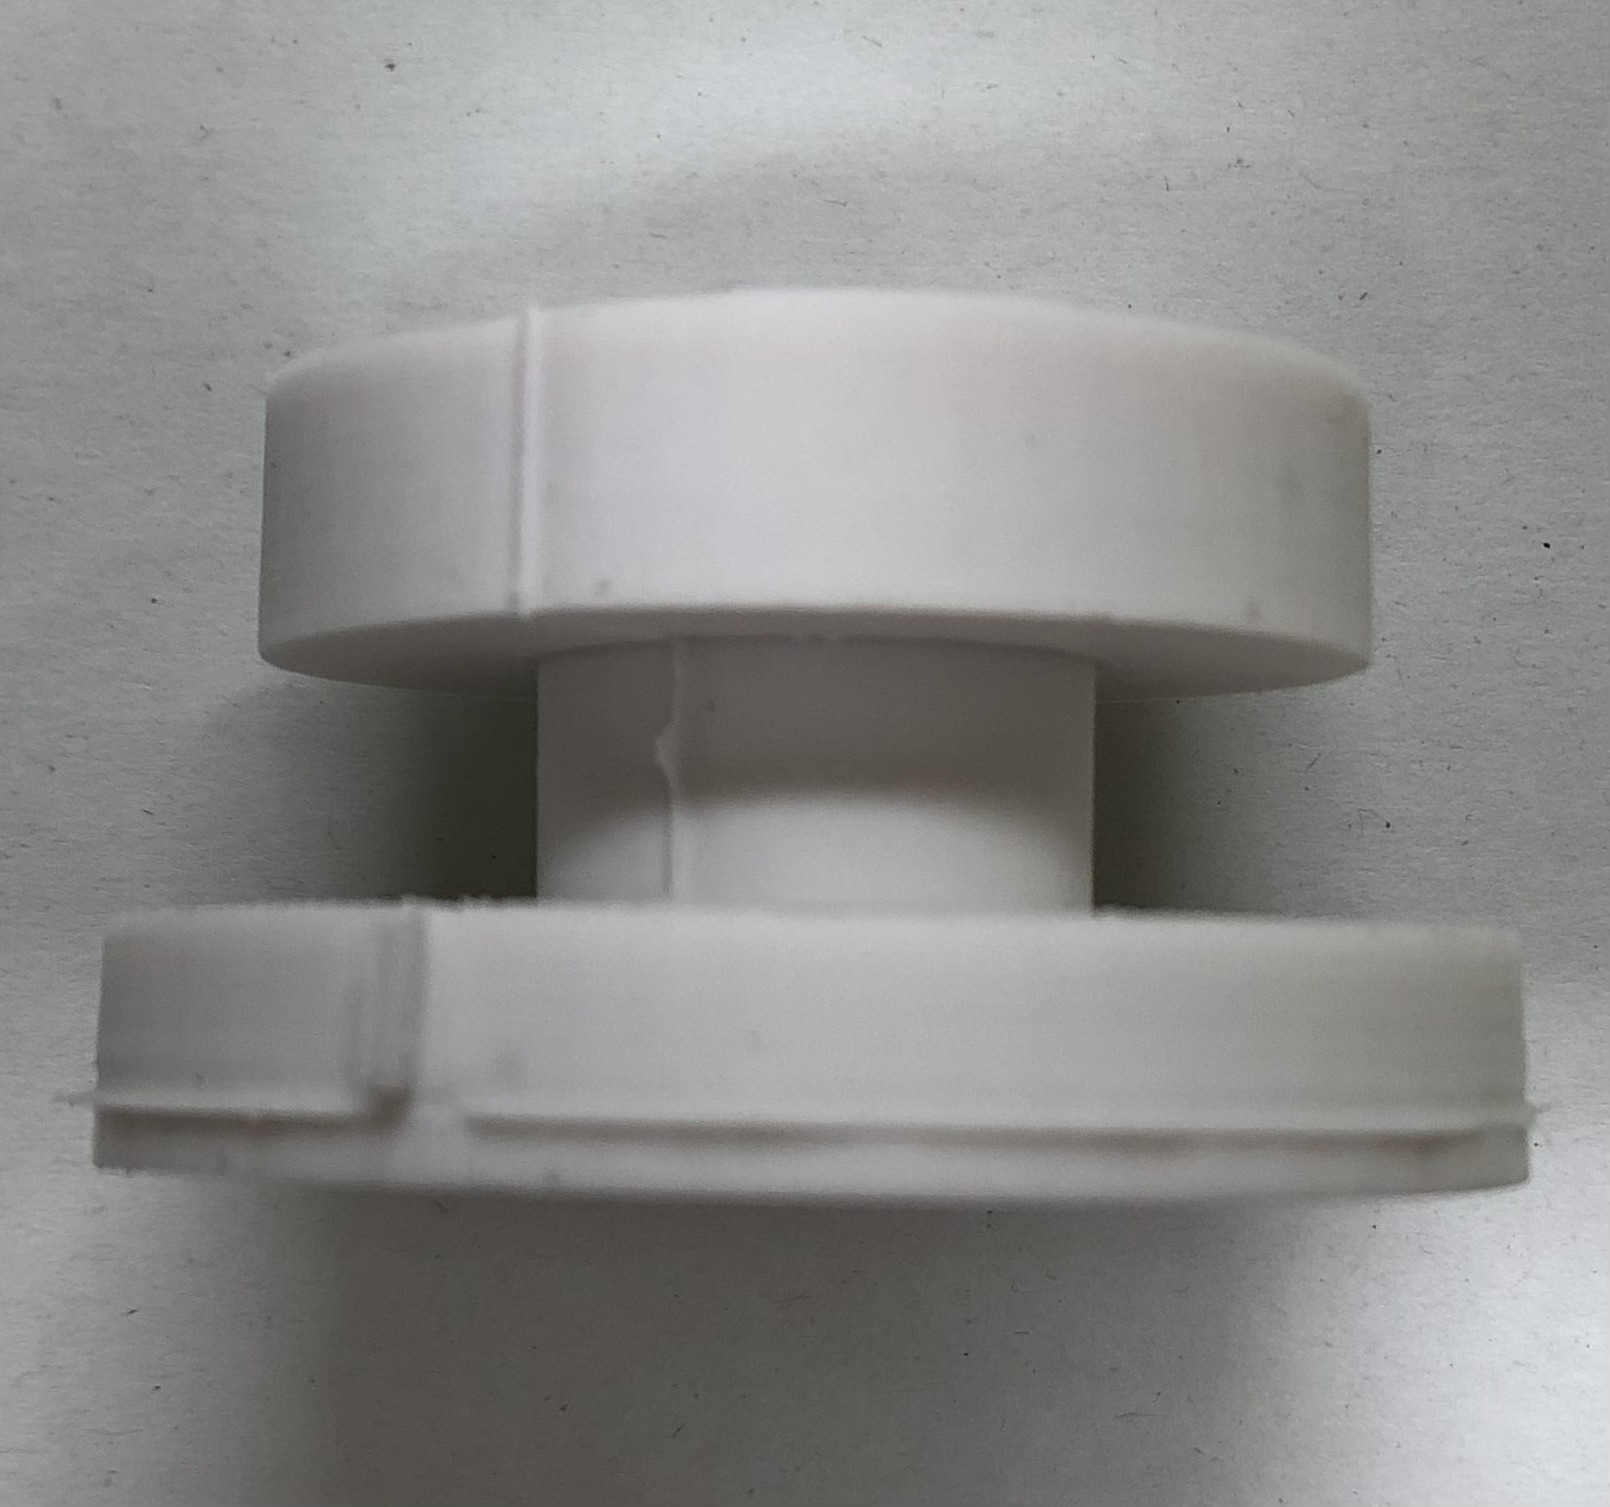
\includegraphics[width=\columnwidth]{./figure/sucker_side.jpg}
      \subcaption{Side view.}
    \end{minipage}
  \end{tabular}
  \caption{Prototype silicon sucker.}
  \label{fig:siliconsucker}
\end{figure}

\subsubsection{接面部の製作}
吸盤による吸着では気密性が極めて重要である\cite{長田勇一2016壁面}.
壁面歩行ロボットを考えるにあたり,吸盤が平らな面に対して吸着能力を発揮することは必須であるが,多少の凹凸面に対しても吸着能力を発揮できなければ,多様な環境での運用は難しい.
そこで先行研究\cite{長田勇一2016壁面}をもとに椀状部の下面にゲル性の接面部を貼ることで凹凸に対しての吸着能力を持たせた.
接面部にはウレタン(Craft Resin社 GUMMY CAST)を用いた.
Fig.~\ref{fig:gelatattchedsucker}に接面部を貼った吸盤の様子を示す.
この接面部を用いて,ピストンで負圧を圧政させる吸着実験を行い,椀状部単体では吸着できなかった約1$\sim$5mmの凹凸を持つ吹き付けタイルに対する吸着を確認することができた.
実験に使用した壁の様子をFig.~\ref{fig:The wall used for the experiment},吸着している様子をFig.\ref{fig:Adsorption experiments on rough surfaces}に示す.

\begin{figure}[t]
    \centering
    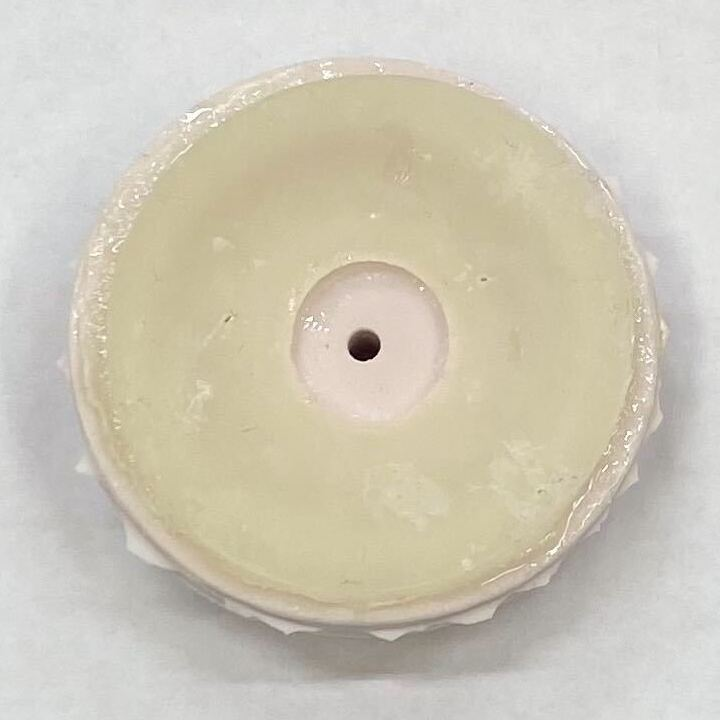
\includegraphics[width=40mm]{./figure/gelsucker.jpg}
    \caption{The sucker atattched to gel.}
    \label{fig:gelatattchedsucker}
\end{figure}

\begin{figure}[b]
    \centering
    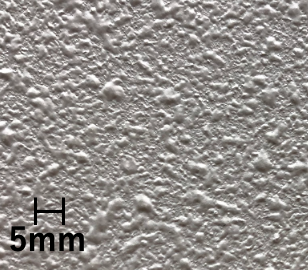
\includegraphics[width=40mm]{./figure/wall}
    \caption{The wall used for the experiment.}
    \label{fig:The wall used for the experiment}
\end{figure}

\begin{figure}[b]
    \centering
    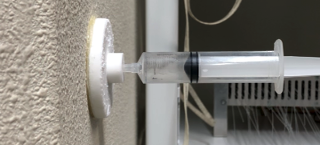
\includegraphics[width=70mm]{./figure/gelsuckerex.PNG}
    \caption{Adsorption experiments on rough surfaces.}
    \label{fig:Adsorption experiments on rough surfaces}
\end{figure}

\begin{comment}
\subsubsection{吸盤の吸着力}
Fig.~\ref{fig:pistonmodel}のように吸盤を簡単にモデル化し,
大気圧を$P_{0}\mathrm{[Pa]}$,吸盤の表面積を$S\mathrm{[m^2]}$としてその吸着力$F\mathrm{[N]}$の理論値を求めた.ただし,吸気前の体積を$V_{0}\mathrm{[m^3]}$,吸気した体積を$V\mathrm{[m^3]}$として,その比を吸気体積比$k$として定めた.

\begin{align}
    F = P_{0}S(1 - \frac{1}{k+1})
    \label{eq:suckerforce}
   \end{align}
   \begin{align}
    k = \frac{V}{V_0}
    \label{eq:suckerforce}
\end{align}

本研究においては吸着力の限界の計測にまでは至らなかったが,0.3MPaの圧縮空気をエジェクタ(ZU07LA)を介して吸着力に変換し,直径50mmの吸盤を用いて1.2kgの物体を持ち上げられる事までは確認した.今後壁面歩行をする機体の重量を考える際に吸着力の値は必要になると考えられるので,その理論計算式をここで示した.

\begin{figure}
    \centering
    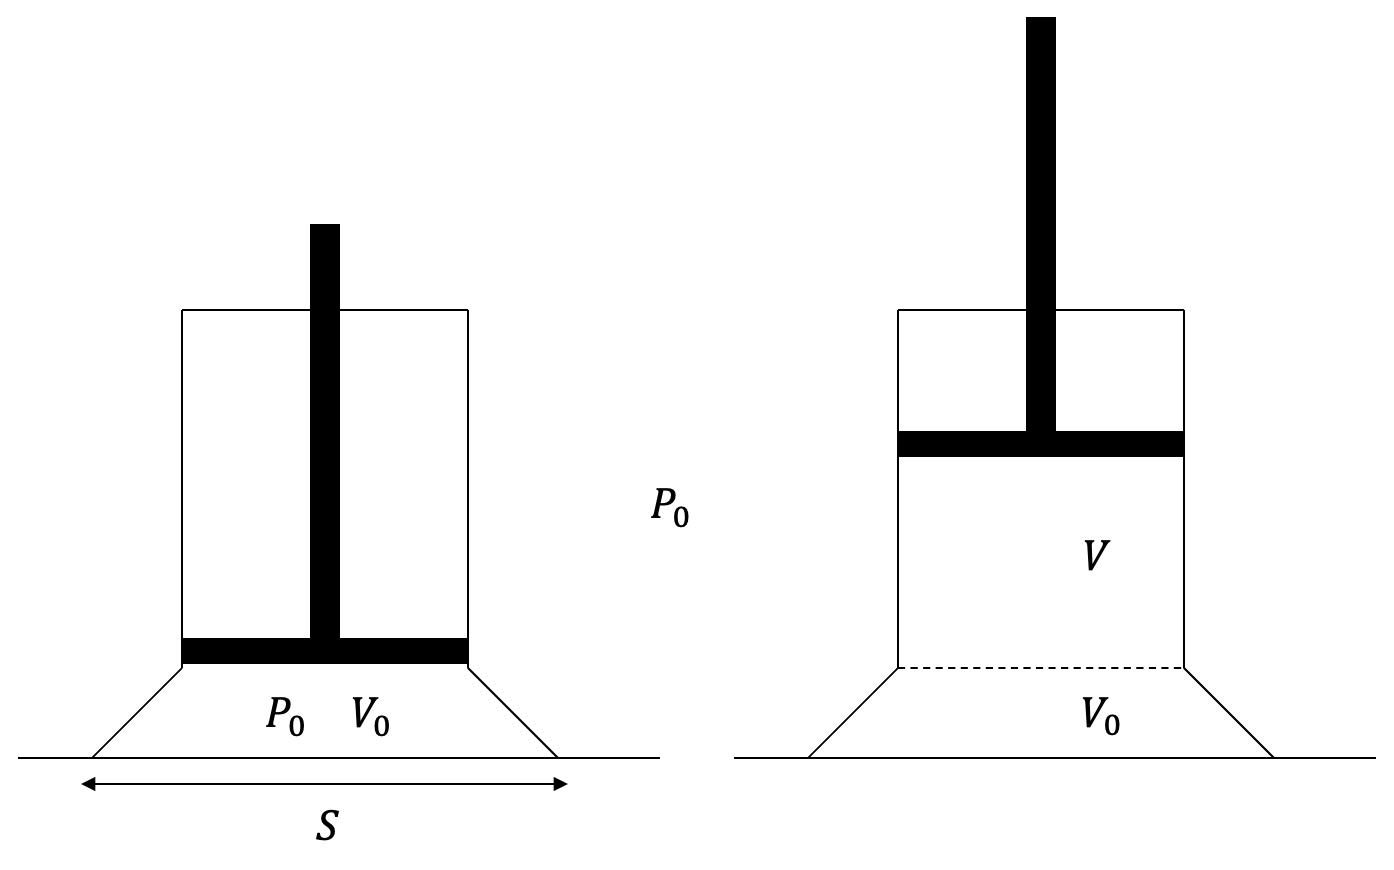
\includegraphics[width=\columnwidth]{./figure/model.png}
    \caption{The model of piston sucker.}
    \label{fig:pistonmodel}
\end{figure}

\end{comment}


\subsection{空気圧による着脱の実現}
歩行を実現するためには単に吸着するだけでなく負圧を大気圧に解放して脱着することも求められる.
そこで電磁弁を用いることで空気の圧縮と大気圧への解放を切り替えられるようにした.
実験においてはコンプレッサにエジェクタを繋いで,空気の吸引を電磁弁によって制御出来るようにした.
Fig.~\ref{fig:System configuration for adsorption experiments}にそのシステム構成を示す.
この実験において吸着力の性能を測るため,コンプレッサから$P=0.3$[MPa]の圧縮空気を発生させ,エジェクタ(ZU07LA)を介して吸着力に変換し,直径$d=$50[mm]の吸盤を用いて,1.2kgの立方体の金属塊の持ち上げ実験を行い,成功した.
Table~\ref{table:parameters}に実験時の各種パラメータの値を示す.

\begin{comment}
また,将来的な機体の小型化のために60mmのダイヤフラムプラムポンプ(TKV27-1-6-0001)を用いても吸着実験を行い,同様に電磁弁で着脱の制御ができることを確認した.
\end{comment}

\begin{figure}
    \centering
    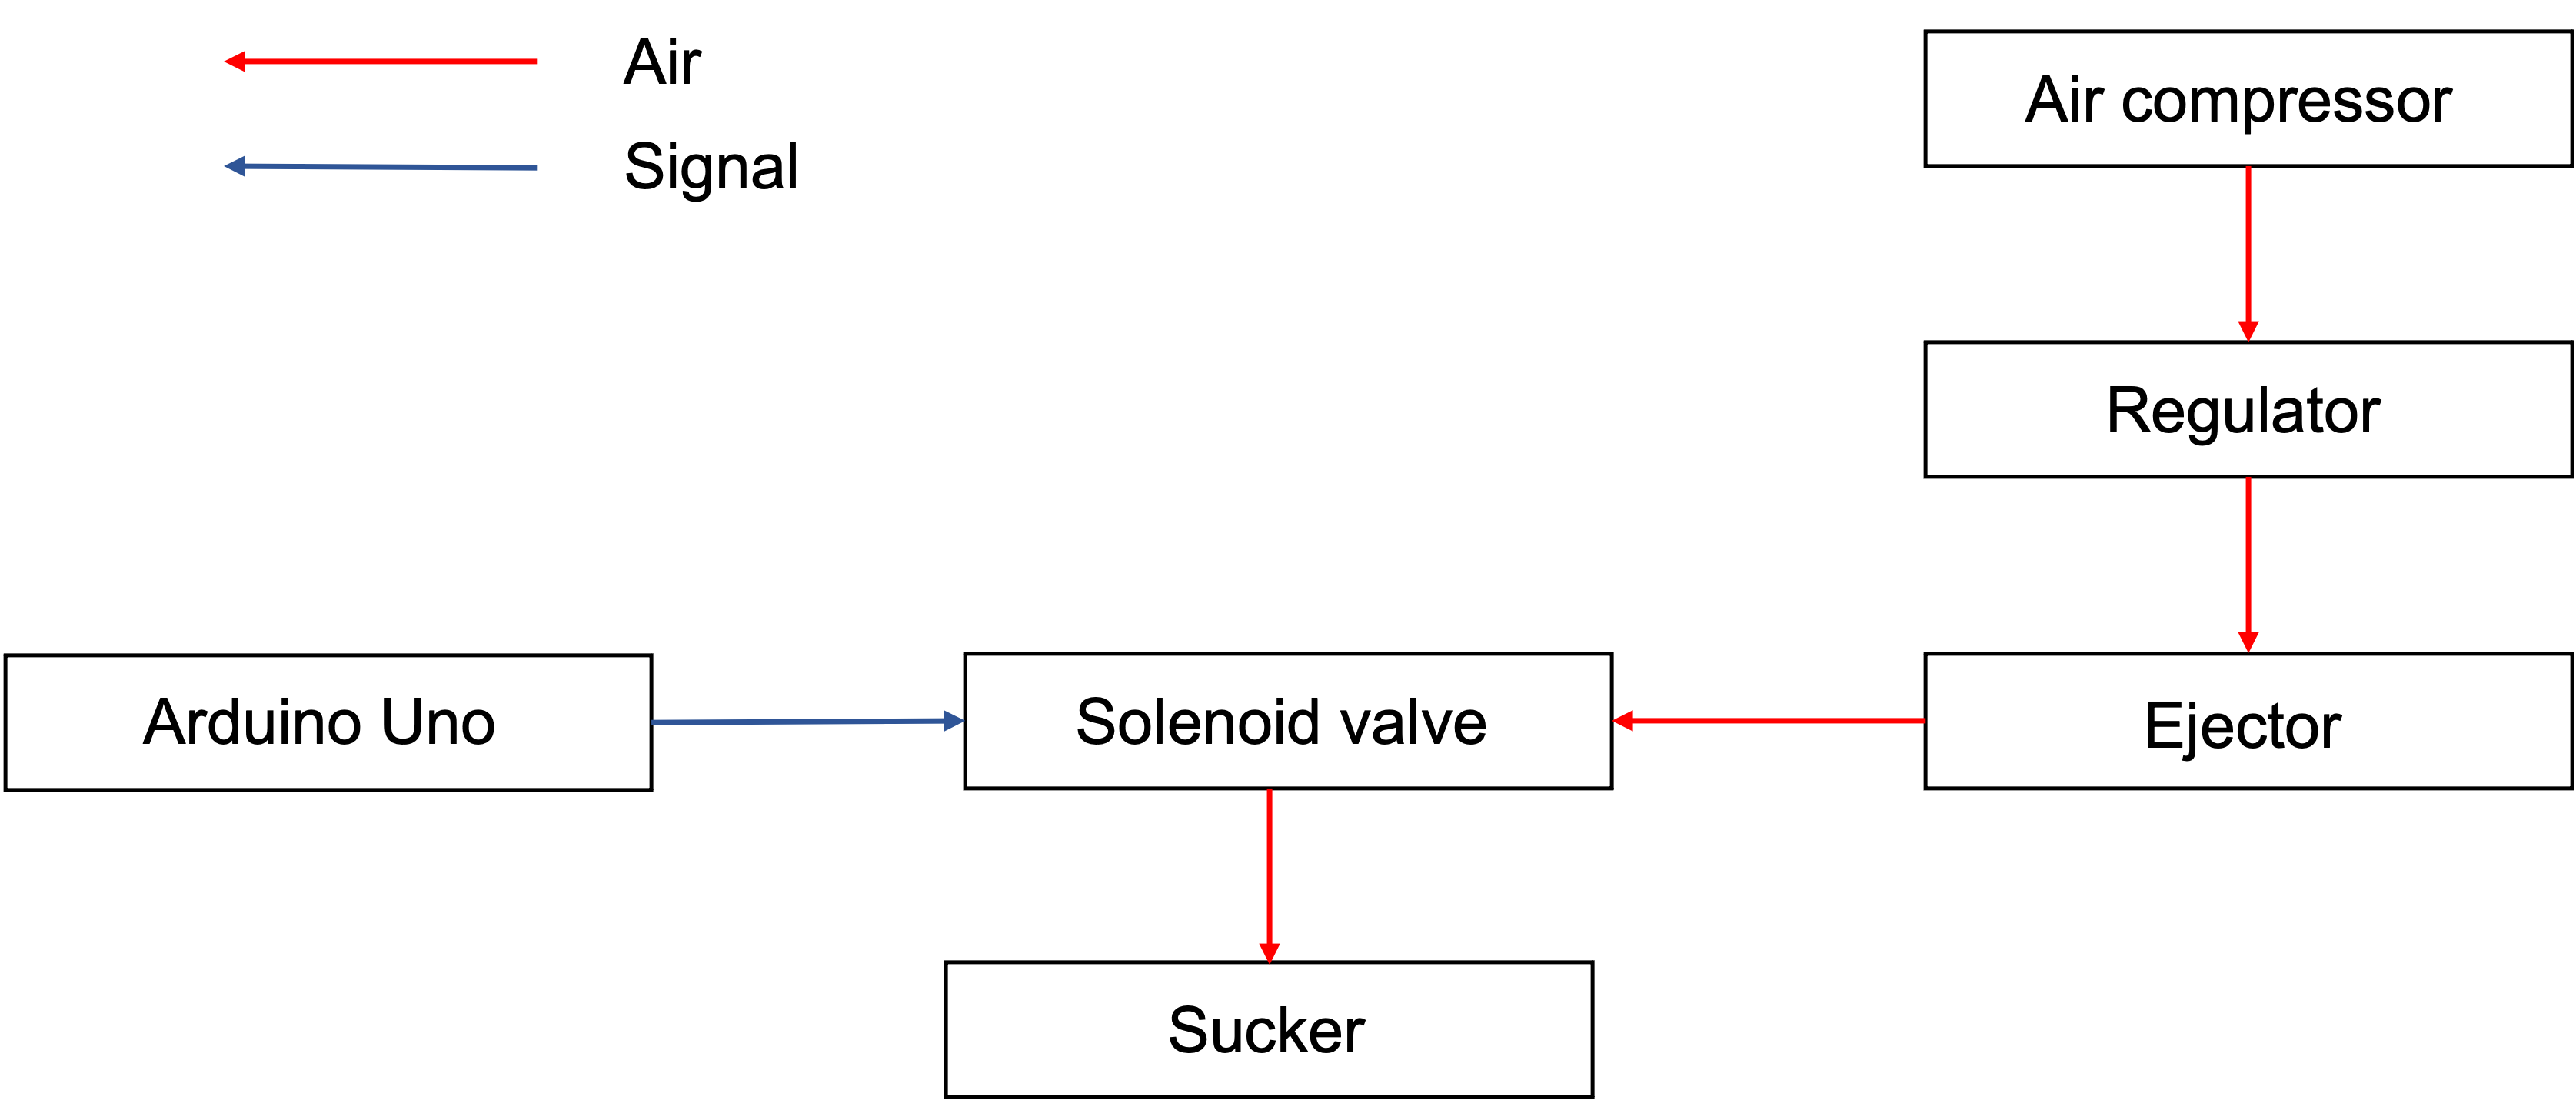
\includegraphics[width=80mm]{./figure/System_configuration_of_adsorption_experiments.png}
    \caption{System configuration of adsorption experiments.}
    \label{fig:System configuration for adsorption experiments}
\end{figure}

\begin{table}
    \caption{Parameters of metal lifting experiment using adsorption mechanism}
     \label{table:parameters}
     \centering
     \begin{tabular}{cc}\hline
      Parameters & Actual values \\ \hline 
     $P$ & 0.3[MPa]\\ 
     $d$ & 60[mm]\\ 
     $m$ & 1.2[kg]\\\hline    
     \end{tabular}
  \end{table}

\section{1関節4足歩行ロボットの製作}
壁面歩行ロボットにおいては,脚を踏み出す際に残った脚の吸着力のみで機体の体重を支えなければいけない.
よって,2脚や3脚では姿勢によって吸着が不安定になる状態が生まれてしまう~\cite{広瀬茂男1991四足壁面移動ロボット}.
また,脚の本数の増加は機体の重量の増加につながるため,できる限り少ない脚で機体を構成するべきである.
以上の点を考慮して4脚を有する機体を製作した.
4足歩行ロボットを製作するにあたって,機体が軽量かつ簡単に歩行を実現できることを目的にファブウォーカー(ELEKIT社)というロボットを参考にした.
このロボットは1関節の4足歩行ロボットで,取り付けられた2つのサーボモータを交互に動かすことで歩行を実現している.
製作においては地面との摩擦力を増やすため,脚先にシリコンの滑り止めをつけた.Fig.~\ref{fig:quadruped_robot}に製作した機体を示す.

歩行動作の実現にあたっては前後のサーボモータを同周期で動かすと,停滞し歩行にならなかったため,時間差をつけることで歩行を実現した.
これは時間差により地面と脚の間に隙間が生まれることで歩行できるようになったからであると考えられる.

制御にあたっては,サーボモータの回転角$\theta$[degree],片方のサーボモータが動いてからもう片方のサーボモータが回転を始めるまでの時間差$t$[ms],1つのサーボモータの回転周期$T$[ms]の3つのパラメータを変更することで様々な歩行形態を確認することができた.
実際に確認できた歩行のうち3パターンの歩行形態を示す.
Table.\ref{table:Parameters_in_quadruped_experiment}に各パターンにおけるパラメータの値を示した.
各パターンにおけるパラメータを用いて4足歩行を行った際の理論的な歩容をGait chartを用いて示す.
Gait chartとは歩行時の接地状態を視覚的に表現した図であり,横軸が経過時間,縦軸が各脚の接地の状態を表す.
Fig.~\ref{fig:Gait_chart_of_quadruped}に各パターンのGait chartを示す.脚の遊脚期を白,支持脚時を黒で表している.また,RFは右前脚,RHは右後脚,LFは左前脚,LHは左後脚を表している.
また,各パターンの実機実験の最初の4歩の様子をFig.~\ref{fig:Quadruped_robot_walking}に示す.


\begin{table}
    \caption{Parameters in quadruped experiment}
     \label{table:Parameters_in_quadruped_experiment}
     \centering
     \begin{tabular}{cccc}\hline
      Pattern & $\theta$ & $t_{df}$ & $T$ \\ \hline 
     1 & 30$^\circ$ & 100[ms] & 1000[ms] \\ 
     2 & 30$^\circ$ & 20[ms] & 100[ms] \\ 
     3 & 40$^\circ$ & 100[ms] & 600[ms] \\ \hline    
     \end{tabular}
  \end{table}

\begin{figure}
    \centering
    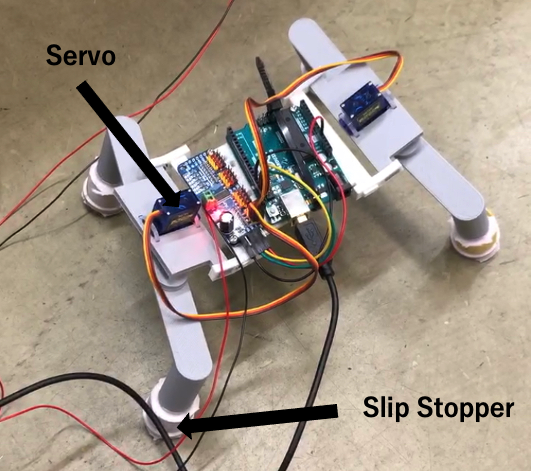
\includegraphics[width=60mm]{./figure/4legbot.png}
    \caption{The quadruped robot.}
    \label{fig:quadruped_robot}
\end{figure}

\begin{figure}[h]
    \centering 
    \begin{tabular}{c}
    \begin{minipage}[t]{1\hsize}
      \centering 
      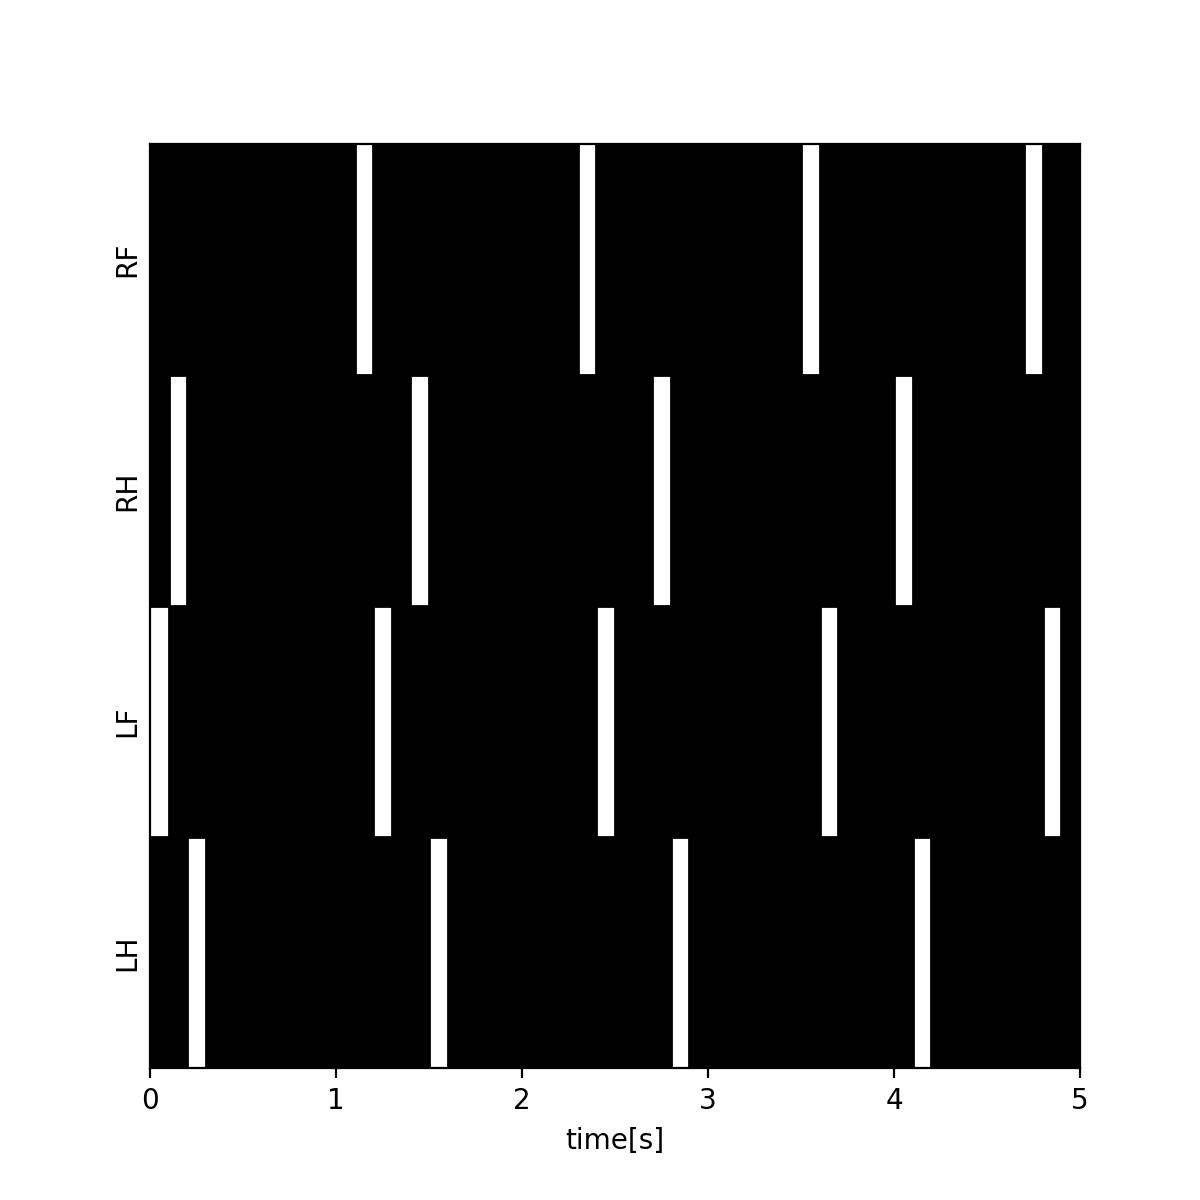
\includegraphics[width=\columnwidth]{./figure/pattern1.png}
      \subcaption{Pattern1.}
    \end{minipage}\\
    \begin{minipage}{1\hsize}
      \centering 
      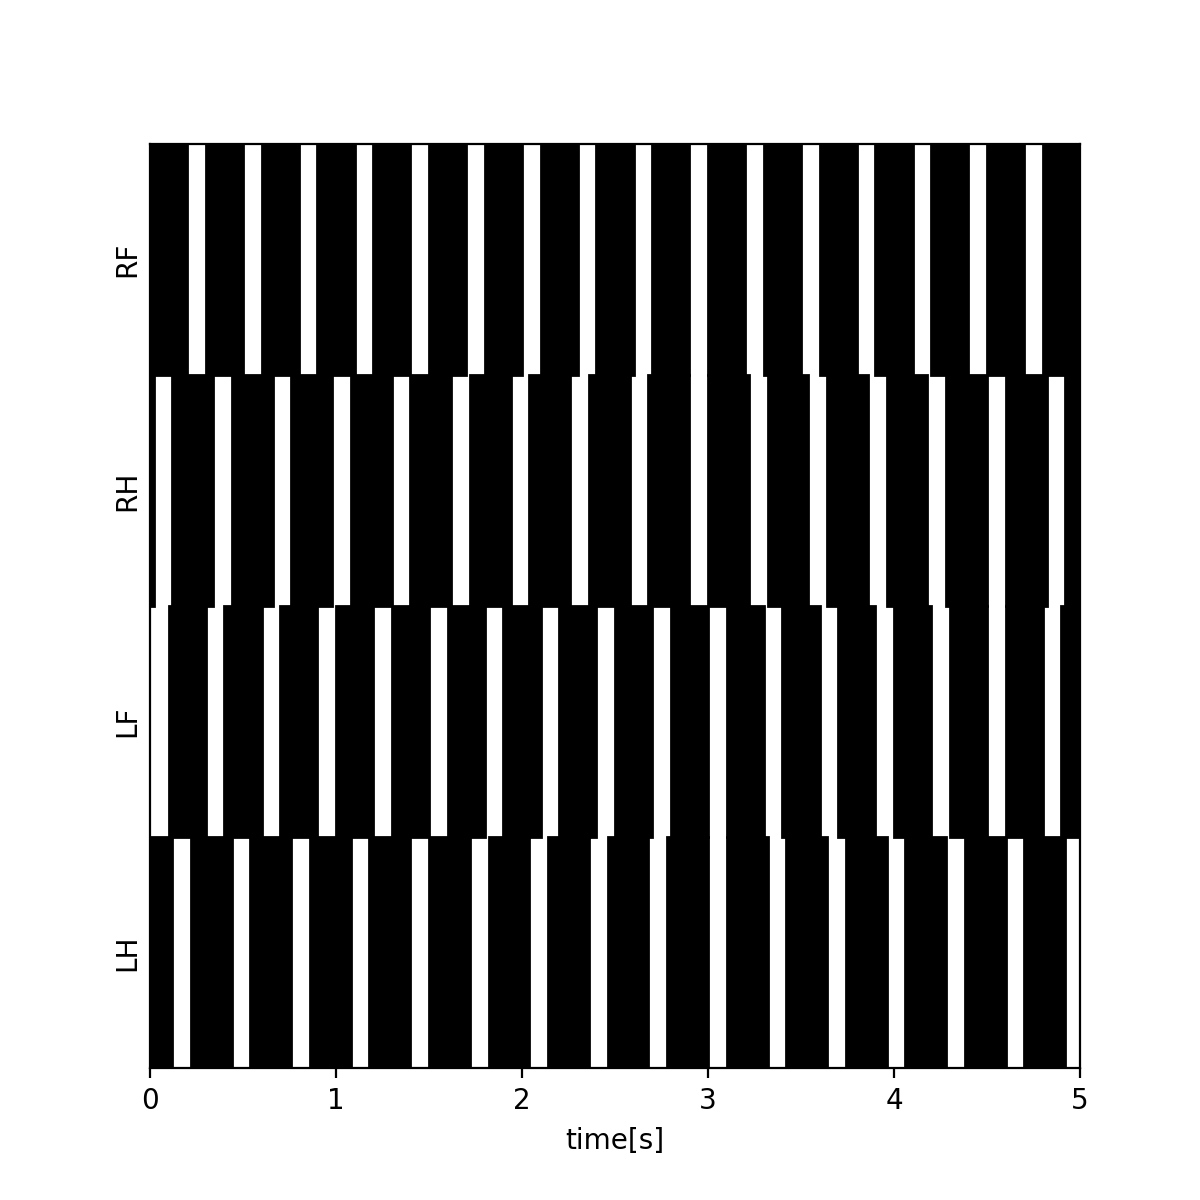
\includegraphics[width=\columnwidth]{./figure/pattern2.png}
      \subcaption{Pattern2.}
    \end{minipage}\\
    \begin{minipage}{1\hsize}
        \centering 
        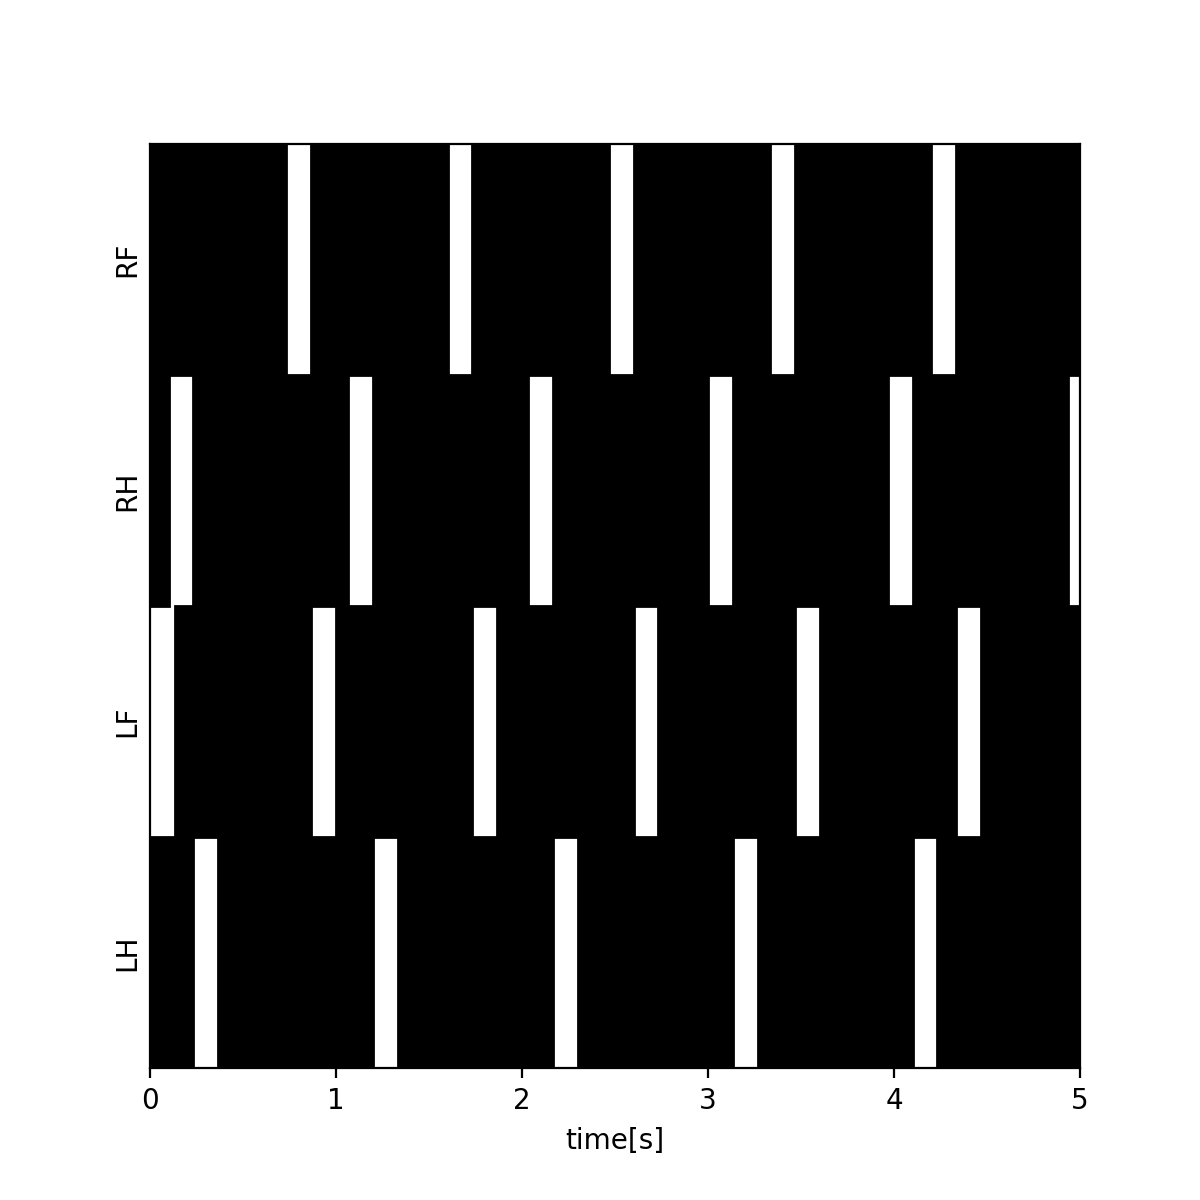
\includegraphics[width=\columnwidth]{./figure/pattern3.png}
        \subcaption{Pattern3.}
      \end{minipage}\\
  \end{tabular}
  \caption{Gait chart of quadruped.}
  \label{fig:Gait_chart_of_quadruped}
\end{figure}

\begin{figure}[h]
    \begin{tabular}{ccc}
    \begin{minipage}{0.33\hsize}
      \centering 
      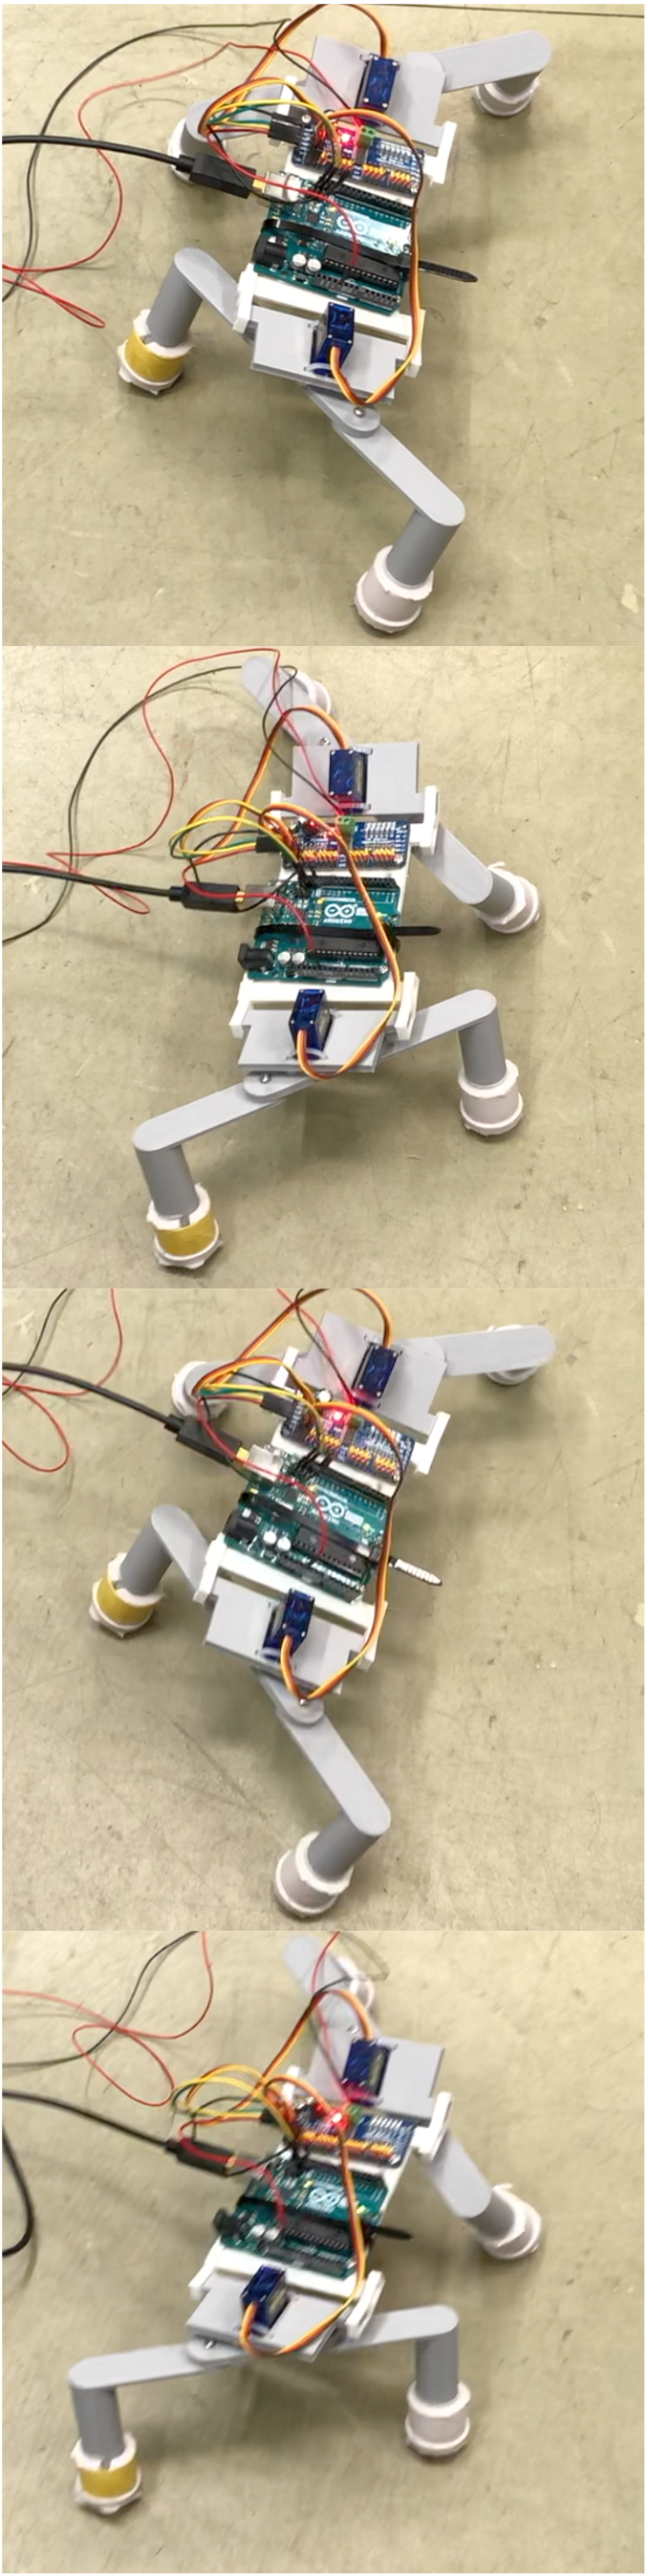
\includegraphics[width=\columnwidth]{./figure/pattern1_real.png}
      \subcaption{pattern1.}
    \end{minipage}
    \begin{minipage}{0.33\hsize}
      \centering 
      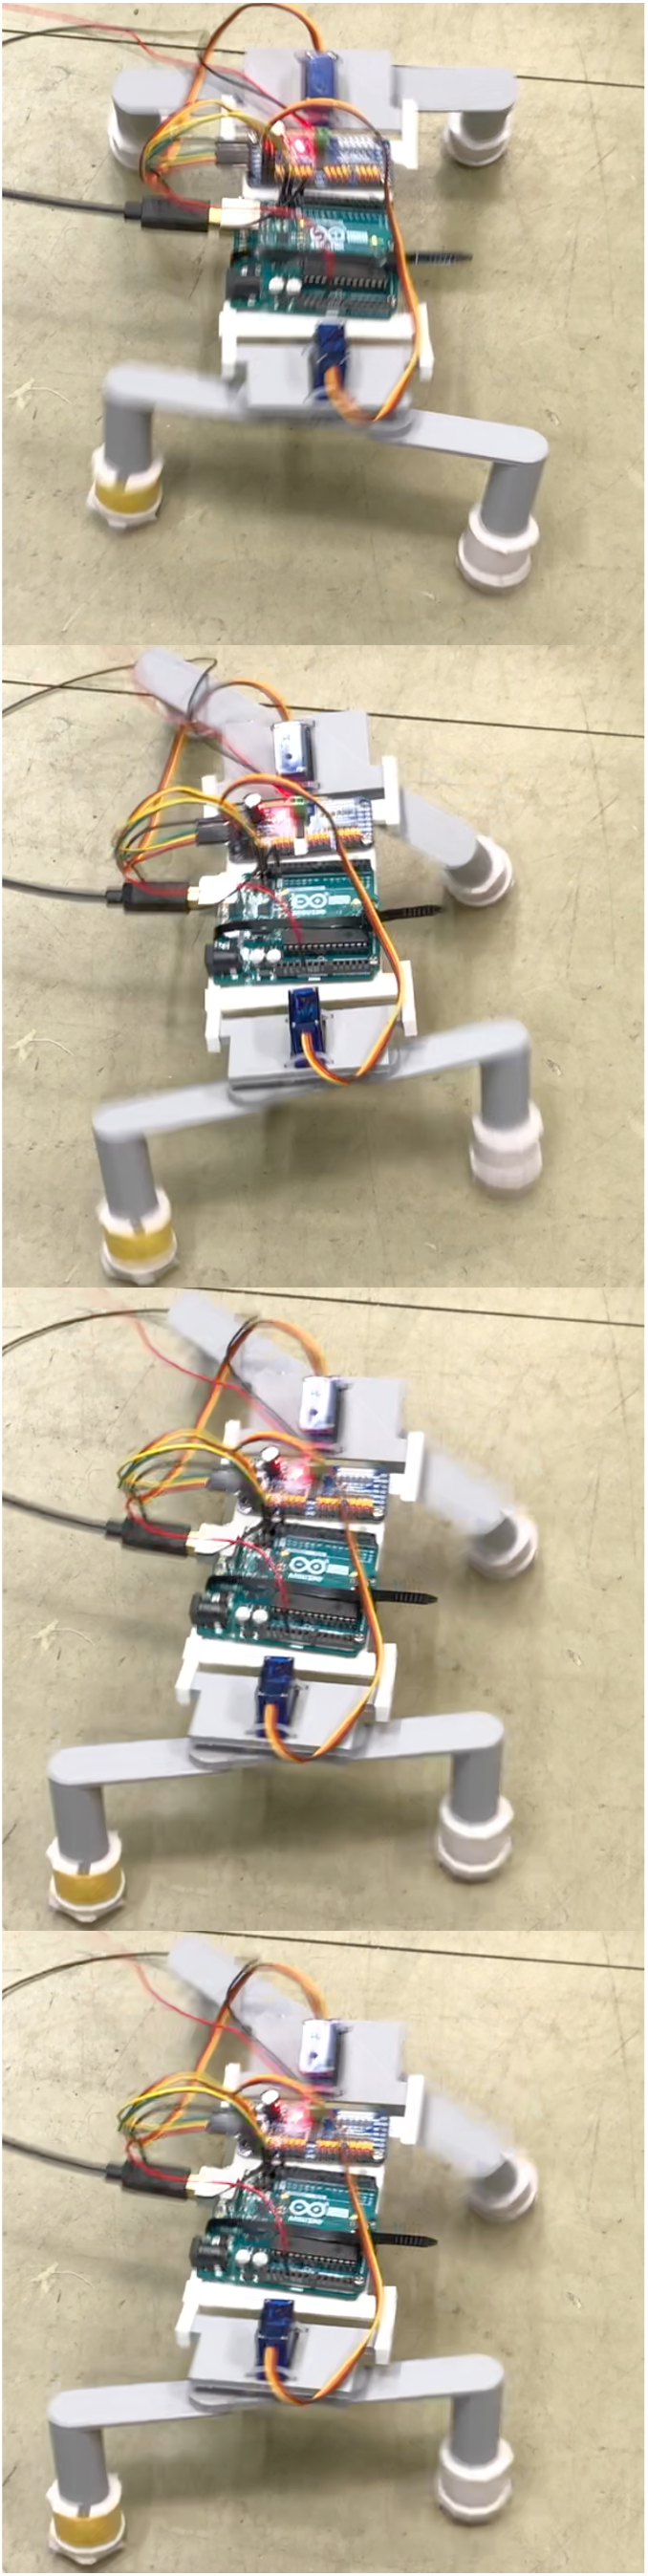
\includegraphics[width=\columnwidth]{./figure/pattern2_real.png}
      \subcaption{pattern2.}
    \end{minipage}
    \begin{minipage}{0.33\hsize}
        \centering 
        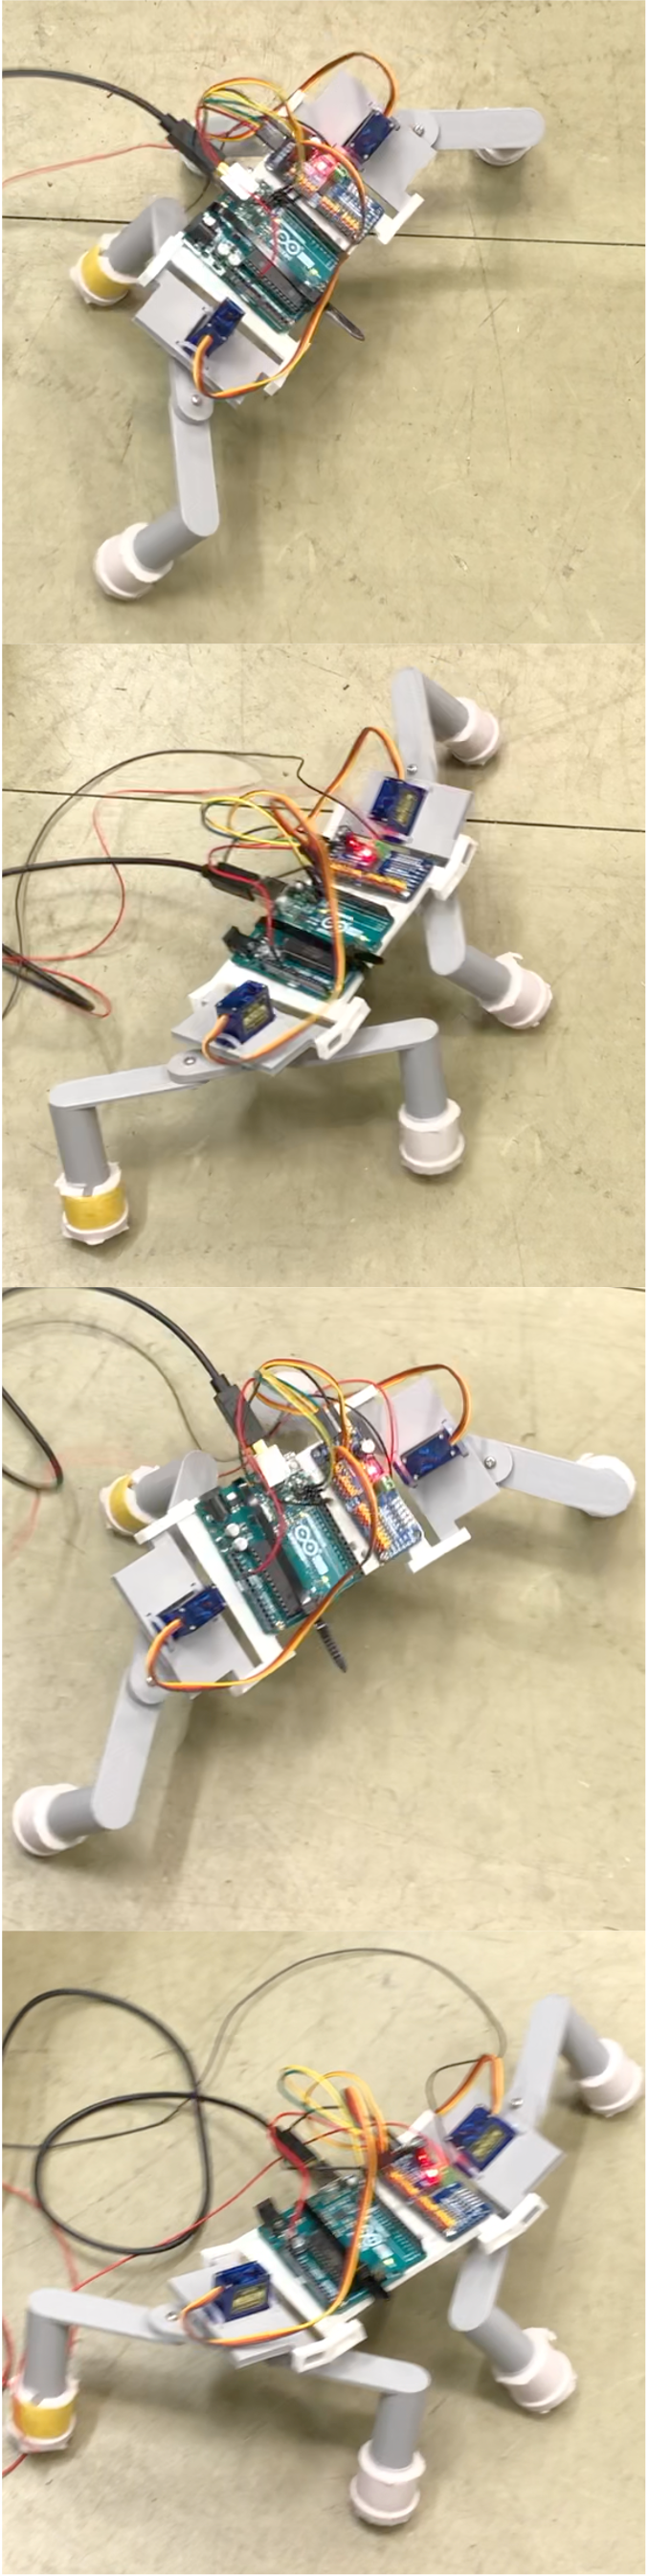
\includegraphics[width=\columnwidth]{./figure/pattern3_reak.png}
        \subcaption{pattern3.}
      \end{minipage}
  \end{tabular}
  \caption{Quadruped robot walking.}
  \label{fig:Quadruped_robot_walking}
\end{figure}

\section{4足歩行ロボットを用いた斜面への吸着実験}
4足歩行ロボットの脚に吸着機構をつけた.製作した機体をFig.~\ref{fig:The_quadruped_with_sucker.}に示す.
この機体を吸着機構によって支持できるか確認するために,アクリル板に対し4脚または2脚で接地しアクリル板を180度回転させて機体が支持できるかの実験を行った.実験の模式図をFig.~\ref{fig:Adsorption_experiments_on_ceilings}に示す.
この実験で2脚でも吸着できることを確認した.
180度回転し地面に背を向けた状態での吸着実験と斜面歩行実験を行った.
吸着実験においては,4点設置に加えてトロット歩行中に起こる2点設置でも吸着し機体が天井に対し吊り下がっている状態でも吸着できることを確認した.

\begin{figure}
    \centering
    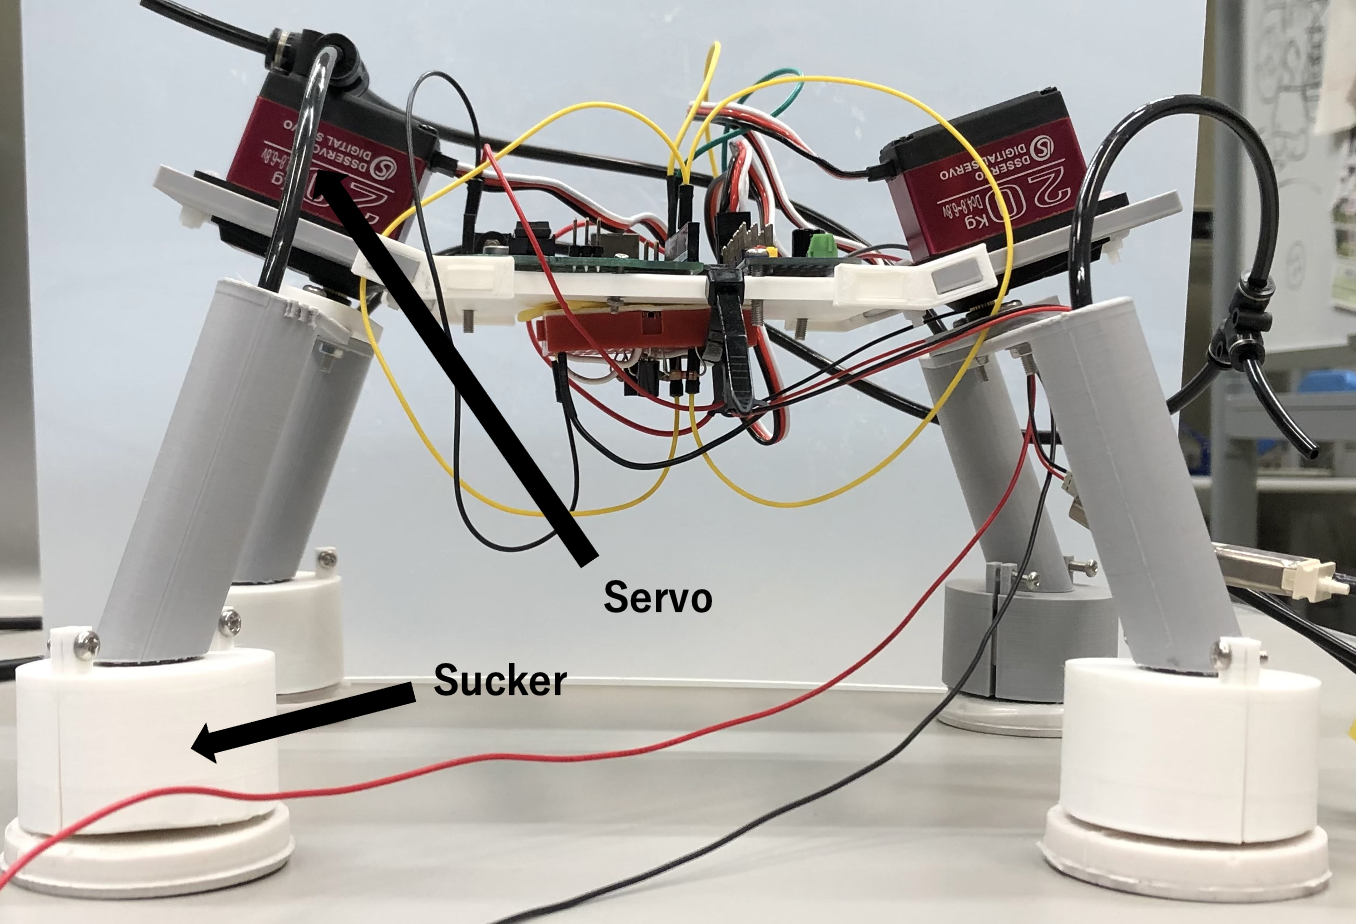
\includegraphics[width=80mm]{./figure/quadruped.png}
    \caption{The quadruped with sucker.}
    \label{fig:The_quadruped_with_sucker.}
\end{figure}


\begin{figure}[h]
    \begin{tabular}{cc}
    \begin{minipage}{0.45\hsize}
      \centering 
      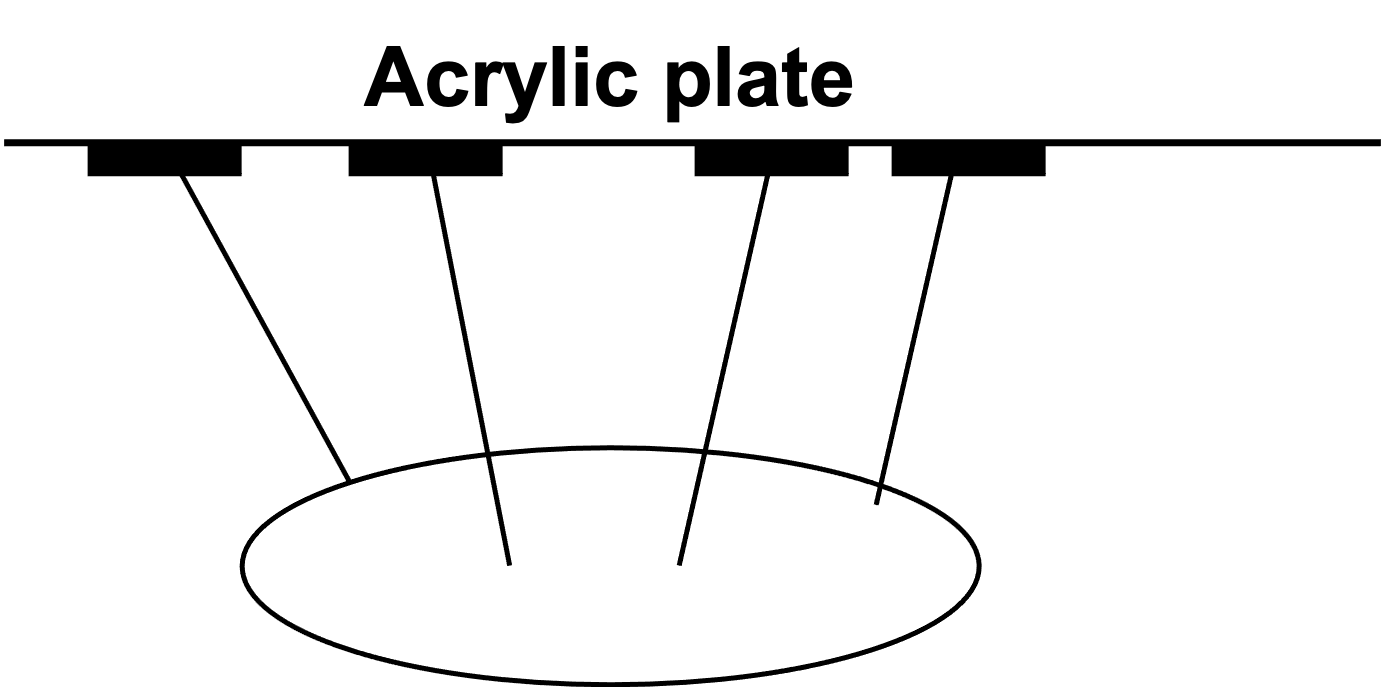
\includegraphics[width=\columnwidth]{./figure/4legs_suck.png}
      \subcaption{4legs.}
    \end{minipage}
    \begin{minipage}{0.45\hsize}
      \centering 
      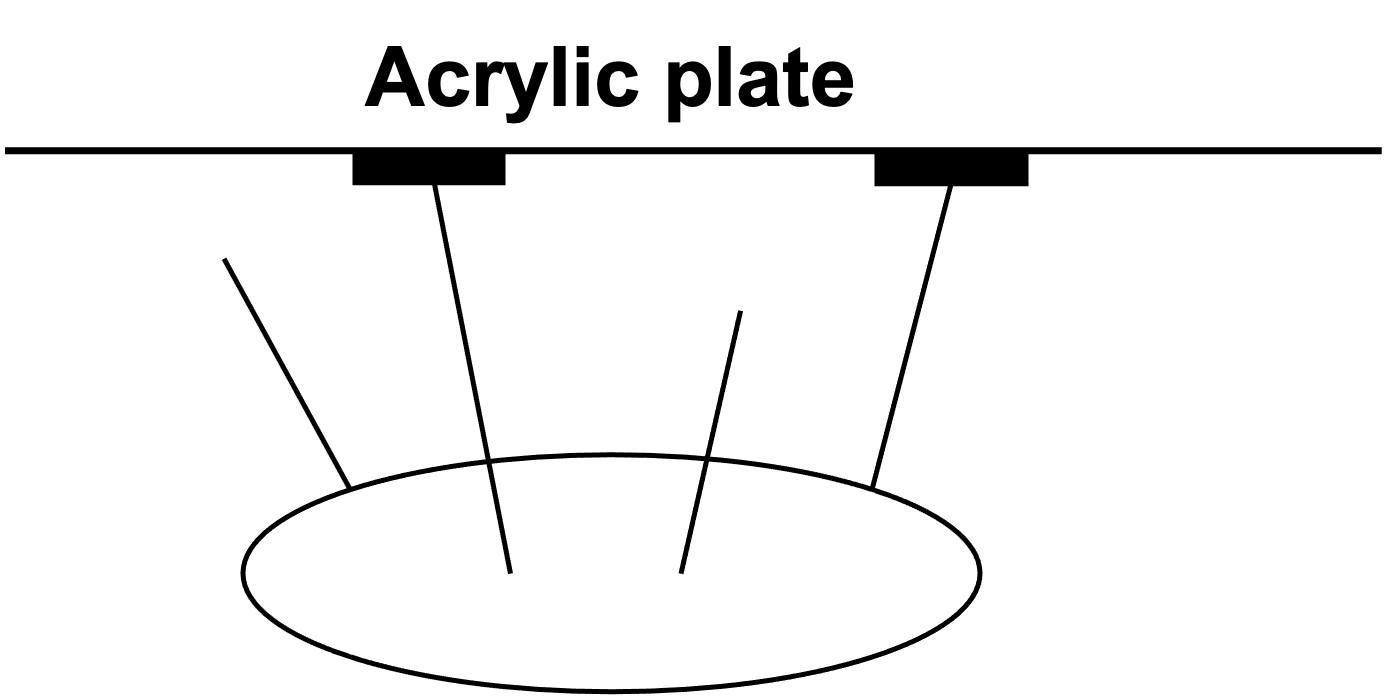
\includegraphics[width=\columnwidth]{./figure/2legs_suck.png}
      \subcaption{2legs.}
    \end{minipage}
  \end{tabular}
  \caption{Adsorption experiments on acrylic plate.}
  \label{fig:Adsorption_experiments_on_ceilings}
\end{figure}

次に滑らかな平面を持つ斜面に対して吸着しながらの歩行実験を行った.
斜面の角度は吸着能力がなければ重力に従って機体がずり落ちる約35度に設定し,4点設置による吸着をした状態から実験を始めた.
この実験では1歩目を踏み出した際に斜面に対して吸着面が浮いてしまい密閉を作ることができなかったため,斜面歩行を実現することはできなかった.

\section{結言}
本研究では空気圧を用いた吸着機構を製作し,それをもとに簡易的な4足歩行の脚型壁面歩行ロボットを製作した.しかしながら斜面での歩行実験において脚を踏み出した際の密閉が確保できず,歩行を実現することができなかった.
今後は,4足歩行ロボットを2関節にすることで吸着面の地面への押し付けを行い壁面歩行を実現することを試みる.

\section{今後の予定}
\begin{itemize}
    \item 2関節の壁面歩行ロボットの設計($\sim$11月下旬)
    \item 2関節壁面歩行ロボットの部品発注・製作(11月下旬$\sim$12月中旬)
    \item 壁面歩行実験(12月中旬)
    \item 卒論書き始め(12月下旬$\sim$)
    \item 卒業発表準備(1月$\sim$)
   \end{itemize}  


{\small
\bibliographystyle{osukalab}
\bibliography{myref}
\clearpage
\end{document}

